% !TeX encoding = UTF-8
\documentclass{beamer}
\usepackage{tikz}
\usepackage[utf8]{inputenc}
\usepackage[spanish]{babel}

\usepackage{smartdiagram}
\usepackage{qtree}
\usepackage{listings}
\lstset{language=Java,
                basicstyle=\footnotesize\ttfamily,
                keywordstyle=\footnotesize\color{blue}\ttfamily,
}
\usetheme{Hannover}
\usecolortheme{crane}
\usepackage{graphicx}
\usepackage{tikz}
\usepackage{hyperref}
\usetikzlibrary{mindmap,backgrounds}

\definecolor{celeste}{HTML}{5E91AA}
\definecolor{azul}{HTML}{163F54}

\setbeamercolor{head1}{fg=celeste}
\setbeamercolor{title}{fg=celeste}
\setbeamercolor{subtitle}{fg=celeste}
\setbeamercolor{frametitle}{fg=celeste}
\setbeamercolor{structure}{fg=azul}
\setbeamercolor{normal text}{fg=azul}


\title{Getting started with Machine Learning}
\author{Víctor Orozco}
\institute{Nabenik}
\date{\today}

\begin{document}

\frame{\titlepage}

\section{Introducción}


\begin{frame}{Víctor Orozco}
    \begin{columns}[T] % contents are top vertically aligned
        \begin{column}[T]{5cm} % each column can also be its own environment
            \begin{itemize}
                \item Developer -JVM, JS- 
                \item Ex becario OAS-GCUB
                \item \href{https://www.oracle.com/javaone/dukes-choice-award.html}{Dukes Choice Award 2016 -GuateJUG-}
                \item \href{http://www.nabenik.com}{CTO/Founder -Nabenik-}
                \item \href{http://www.url.edu.gt/}{Profesor universitario -Universidad Rafael Landivar-}
                \item \href{https://twitter.com/tuxtor}{@tuxtor}
                \item \href{http://vorozco.com}{The J*} 
            \end{itemize}
        \end{column}
        \begin{column}[T]{3cm} % alternative top-align that's better for graphics
            \begin{figure}
                \centering
                
\includegraphics[width=0.6\linewidth]{Images/logos}
            \end{figure}
            
        \end{column}
    \end{columns}
\end{frame}

\subsection{Inteligencia Artificial}
\begin{frame}{Inteligencia Artificial}
    \begin{center}
        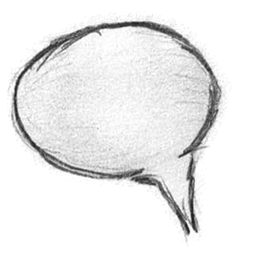
\includegraphics[width=0.4\linewidth]{Images/comment}
    \end{center}
\end{frame}


\begin{frame}{Inteligencia Artificial}
    \begin{center}
        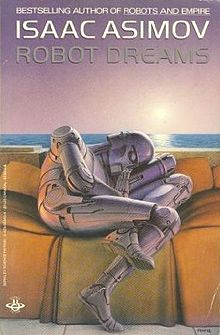
\includegraphics[width=0.4\linewidth]{Images/RobotDreams}
    \end{center}
\end{frame}

\begin{frame}{Inteligencia Artificial}
    \begin{itemize}
        \item \textbf{Entender y construir} entidades 
        inteligentes.
        \item Primeros pasos en robótica
        \item Programas que puedan/sepan reaccionar ante incertezas (CS)
    \end{itemize}
\end{frame}

\begin{frame}{Ramas clásicas}
    \begin{center}
        \begin{tikzpicture}[scale=0.6, transform shape]
        \path[mindmap,concept color=blue,text=white,
        level 1 concept/.append style=
        {every child/.style={concept color=blue!70},sibling angle=-30}]
        node[concept] {IA}
        [clockwise from=0]
        child[concept color=red] { node[concept] {Procesamiento de lenguajes} }
        child[concept color=blue] { node[concept] {Aprendizaje de maquina y mineria de datos}}
        child[concept color=orange] { node[concept] {Visión por computador}}
        child[concept color=red] { node[concept] {Planeamiento} }
        child[concept color=blue] { node[concept] {Representación del conocimiento} }
        child[concept color=orange] { node[concept] {Razonamiento y toma de decisiones} }
        child[concept color=red] { node[concept] {Strong AI} }
        child[concept color=blue] { node[concept] {Robótica} };
        \end{tikzpicture}
    \end{center}
\end{frame}

\begin{frame}{Ramas clásicas}
    \begin{center}
        \begin{tikzpicture}[scale=0.6, transform shape]
        \path[mindmap,concept color=blue,text=white,
        level 1 concept/.append style=
        {every child/.style={concept color=blue!70},sibling angle=-30}]
        node[concept] {IA}
        [clockwise from=0]
        child[concept color=red] { node[concept] {Procesamiento de lenguajes} }
        child[concept color=orange] { node[concept] {Aprendizaje de maquina y mineria de datos}}
        child[concept color=red] { node[concept] {Visión por computador}}
        child[concept color=red] { node[concept] {Planeamiento} }
        child[concept color=red] { node[concept] {Representación del conocimiento} }
        child[concept color=red] { node[concept] {Razonamiento y toma de decisiones} }
        child[concept color=red] { node[concept] {Strong AI} }
        child[concept color=red] { node[concept] {Robótica} };
        \end{tikzpicture}
    \end{center}
\end{frame}

\subsection{Motivación}
\begin{frame}
    \begin{center}
        \large ¿Porqué?
    \end{center}
\end{frame}
\begin{frame}{Motivación}
    \begin{center}
        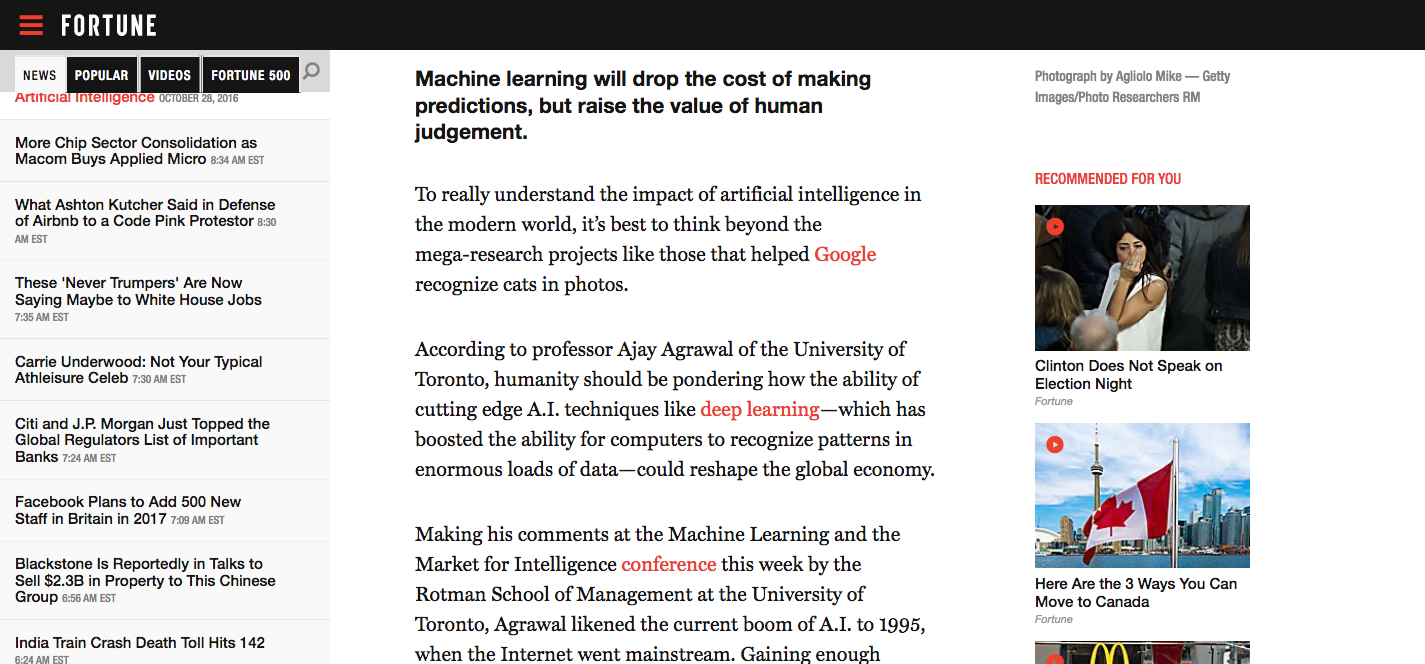
\includegraphics[width=\linewidth]{Images/ml1}
    \end{center}
\end{frame}

\begin{frame}{Motivación}
    \begin{center}
        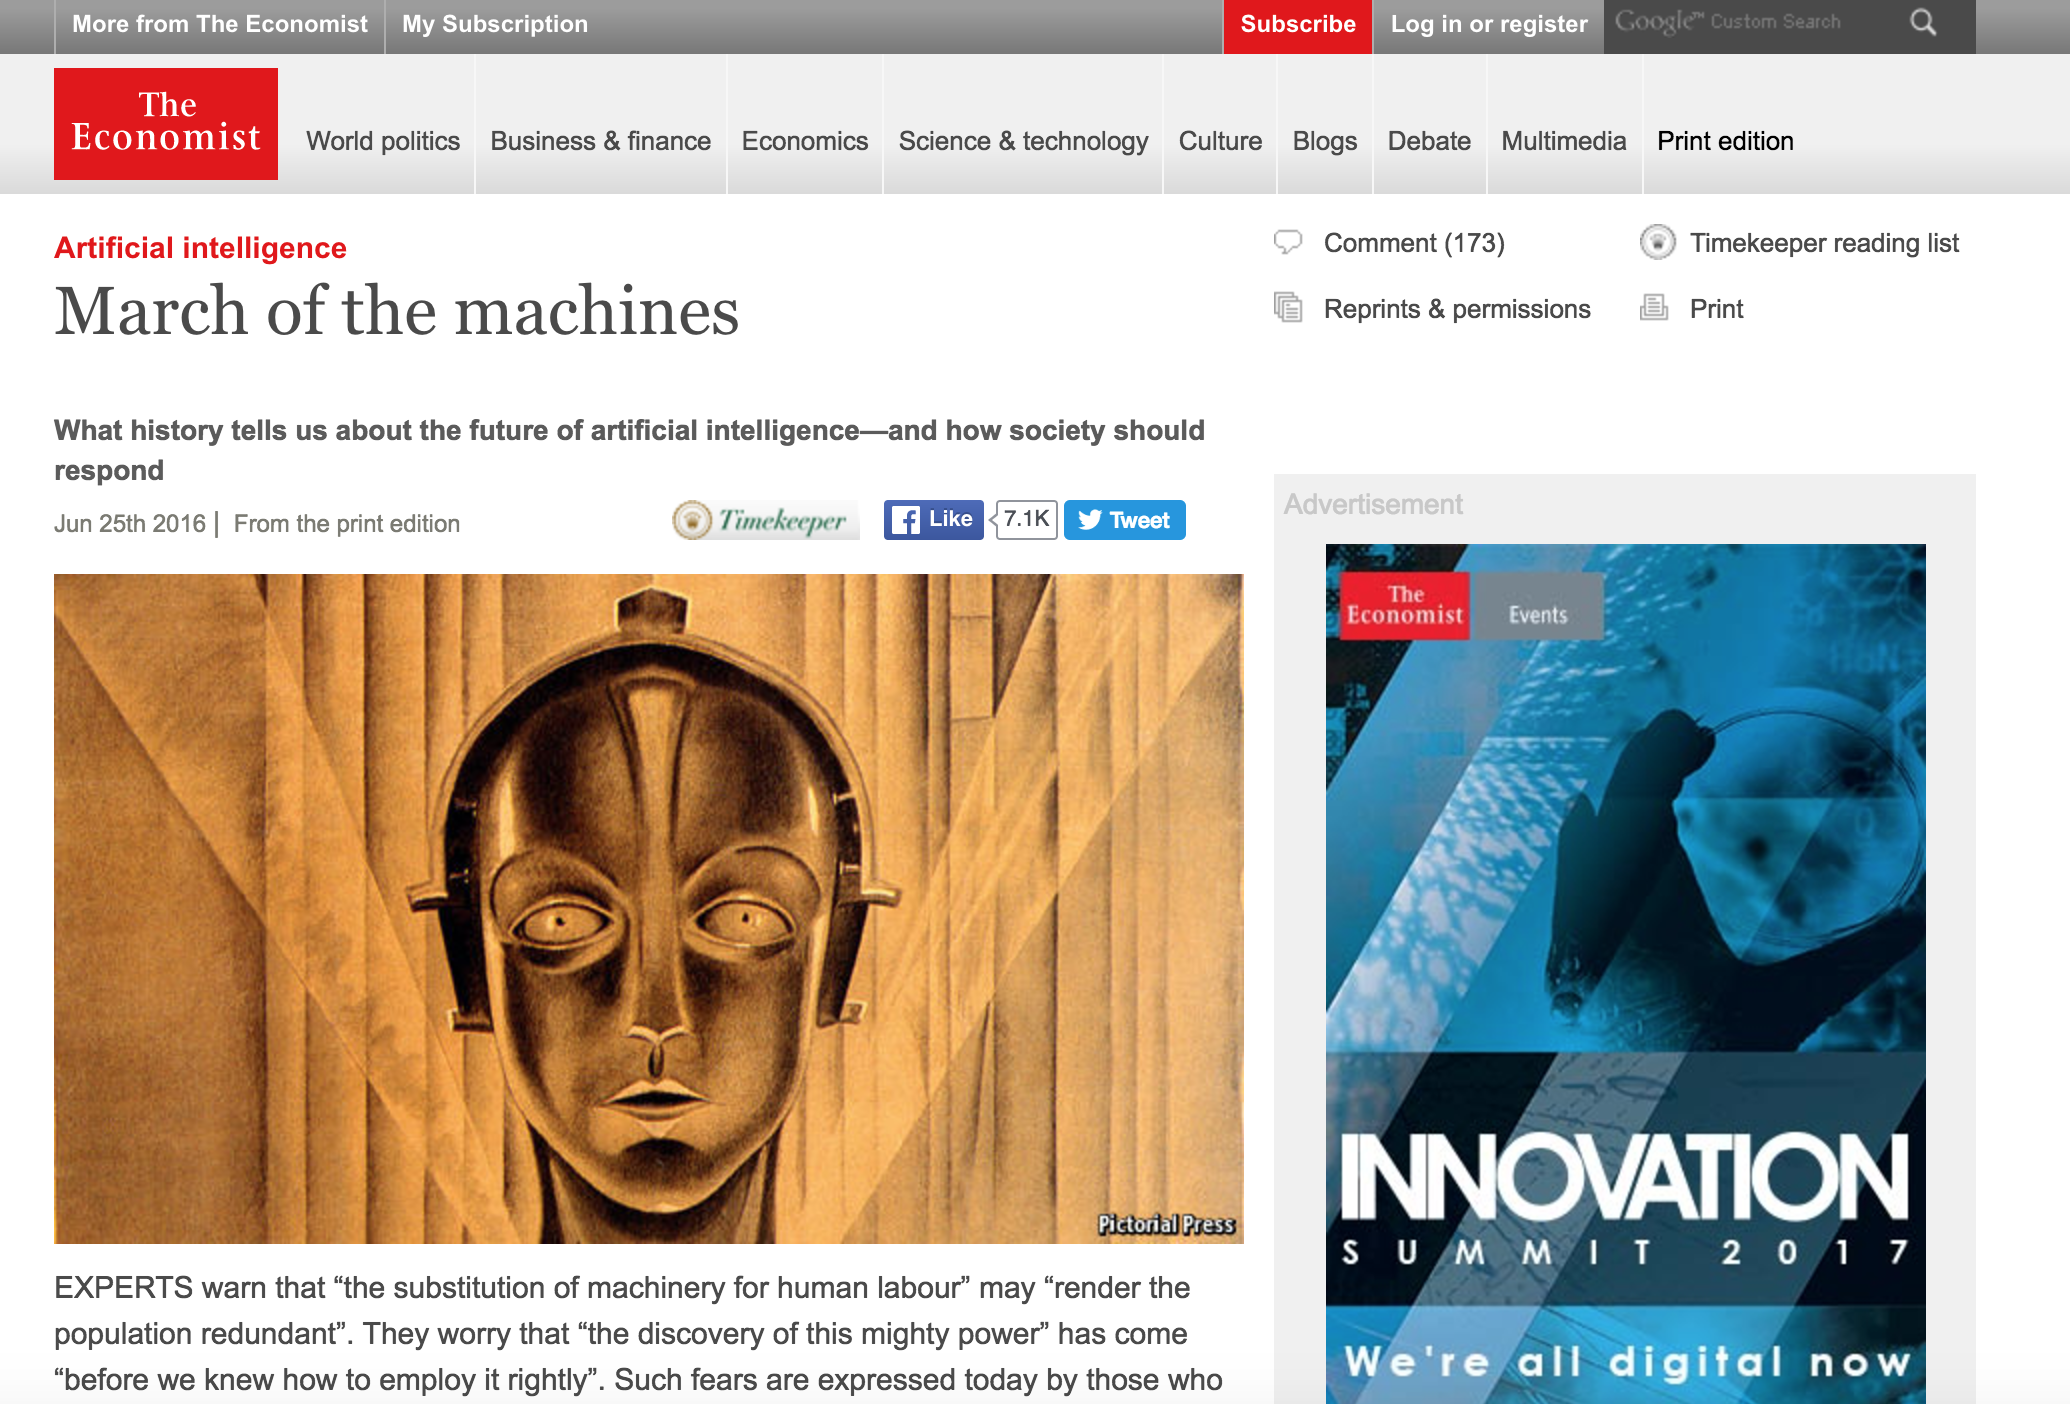
\includegraphics[width=\linewidth]{Images/ml2}
    \end{center}
\end{frame}

\begin{frame}{Motivación}
    \begin{center}
        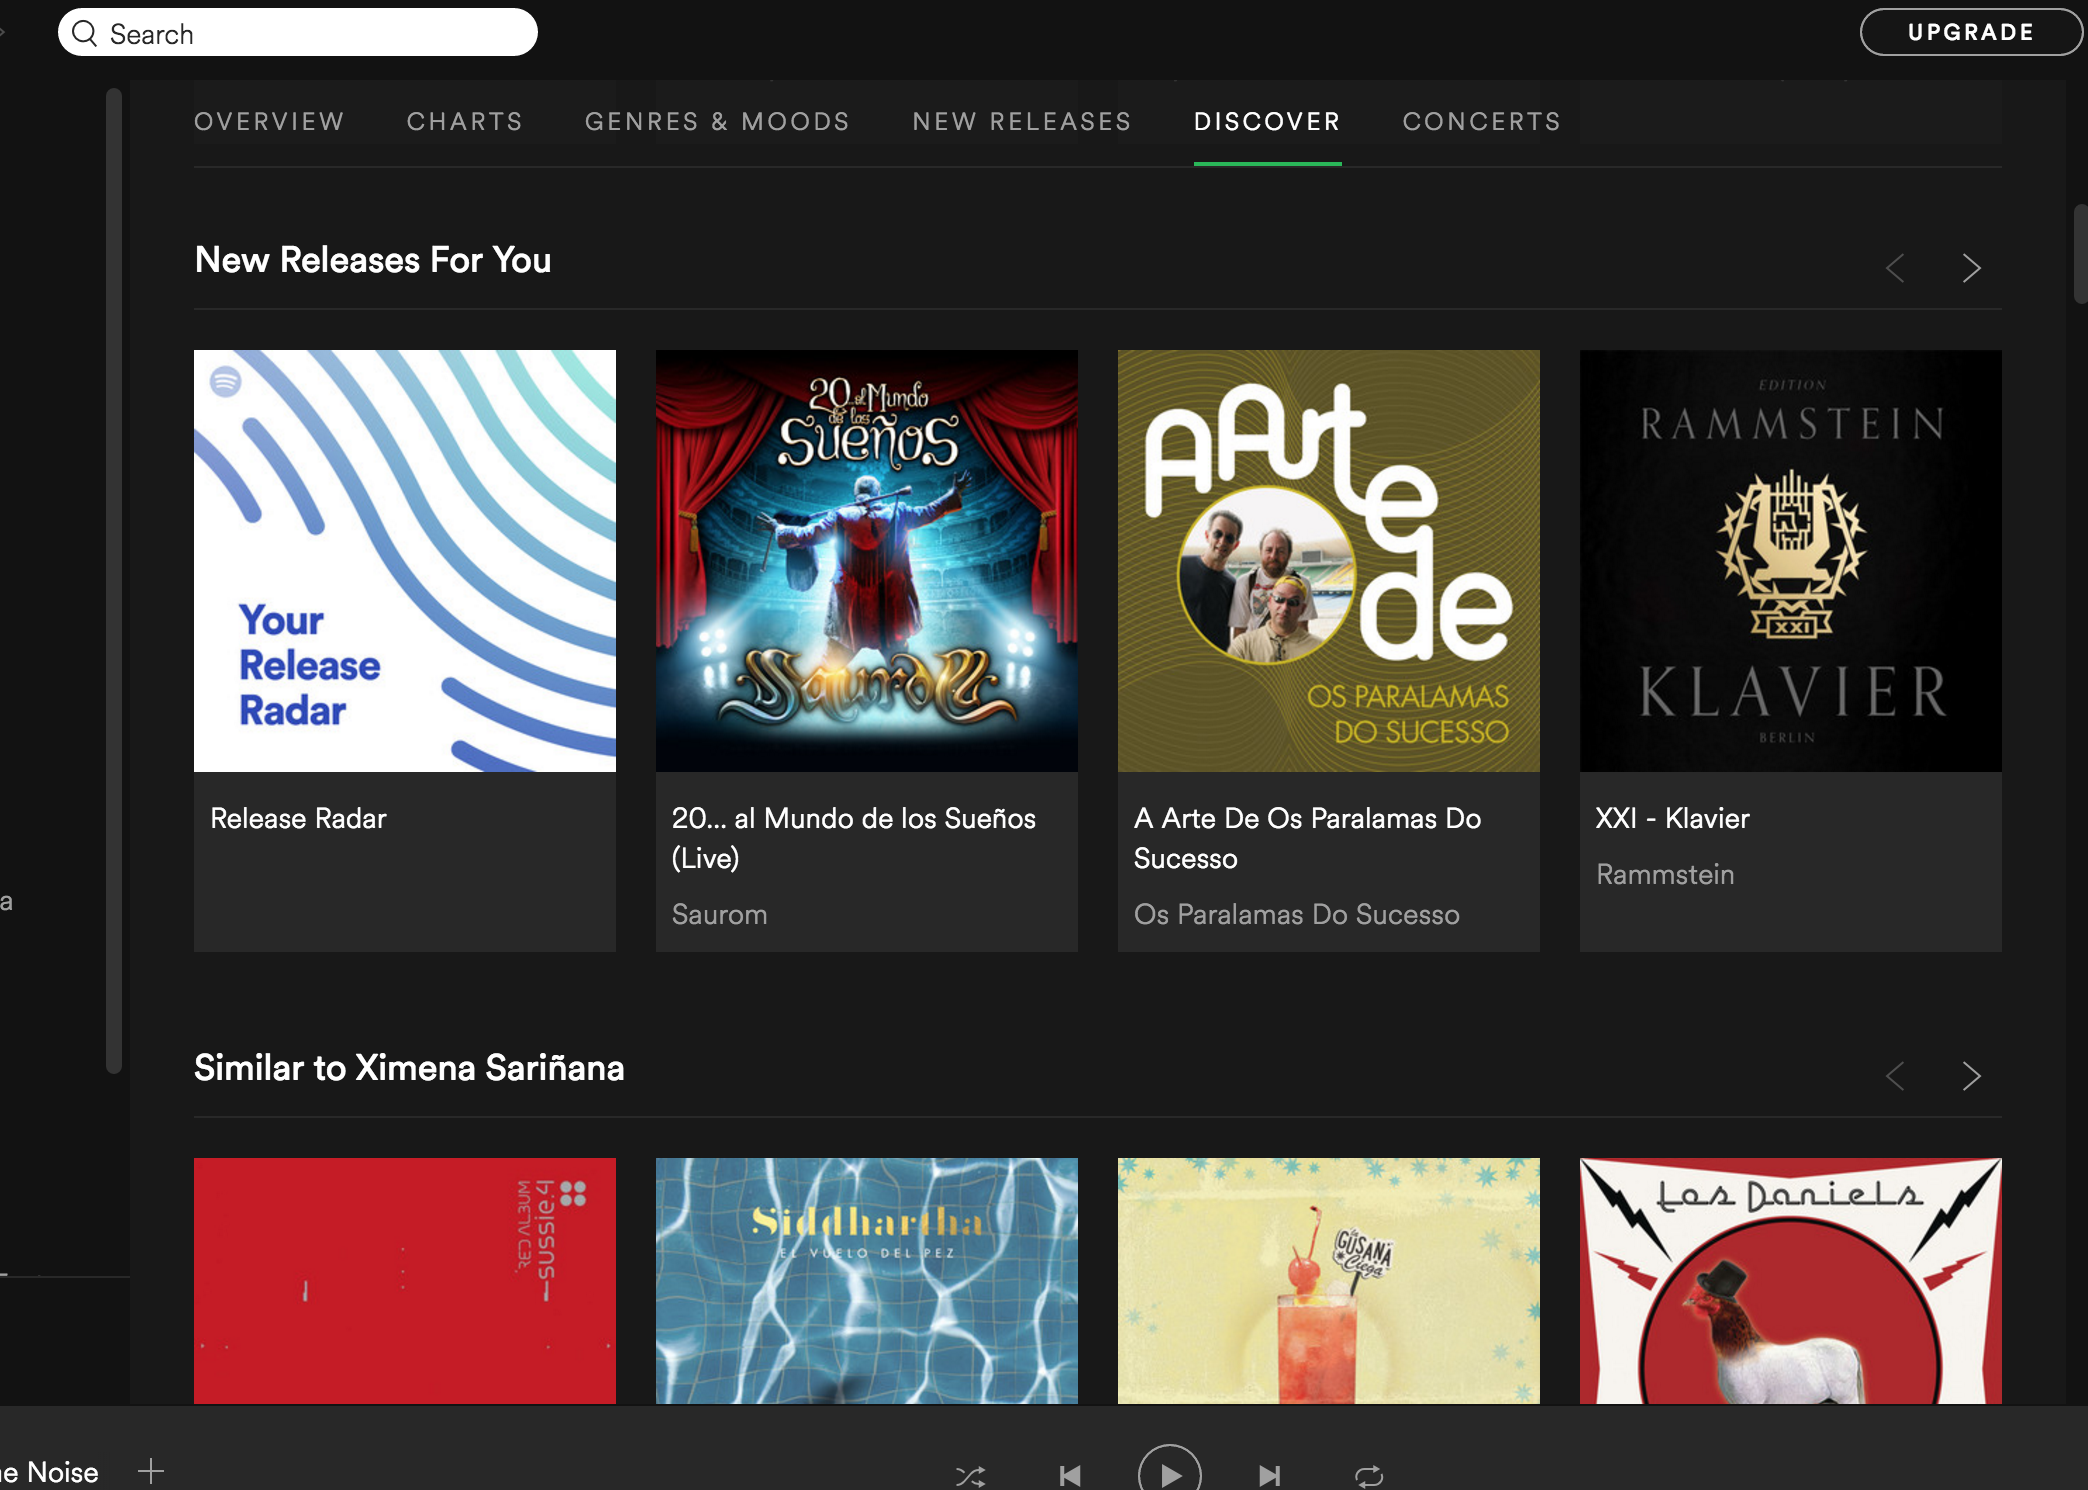
\includegraphics[width=\linewidth]{Images/ml4}
    \end{center}
\end{frame}

\begin{frame}{Motivación}
    \begin{center}
        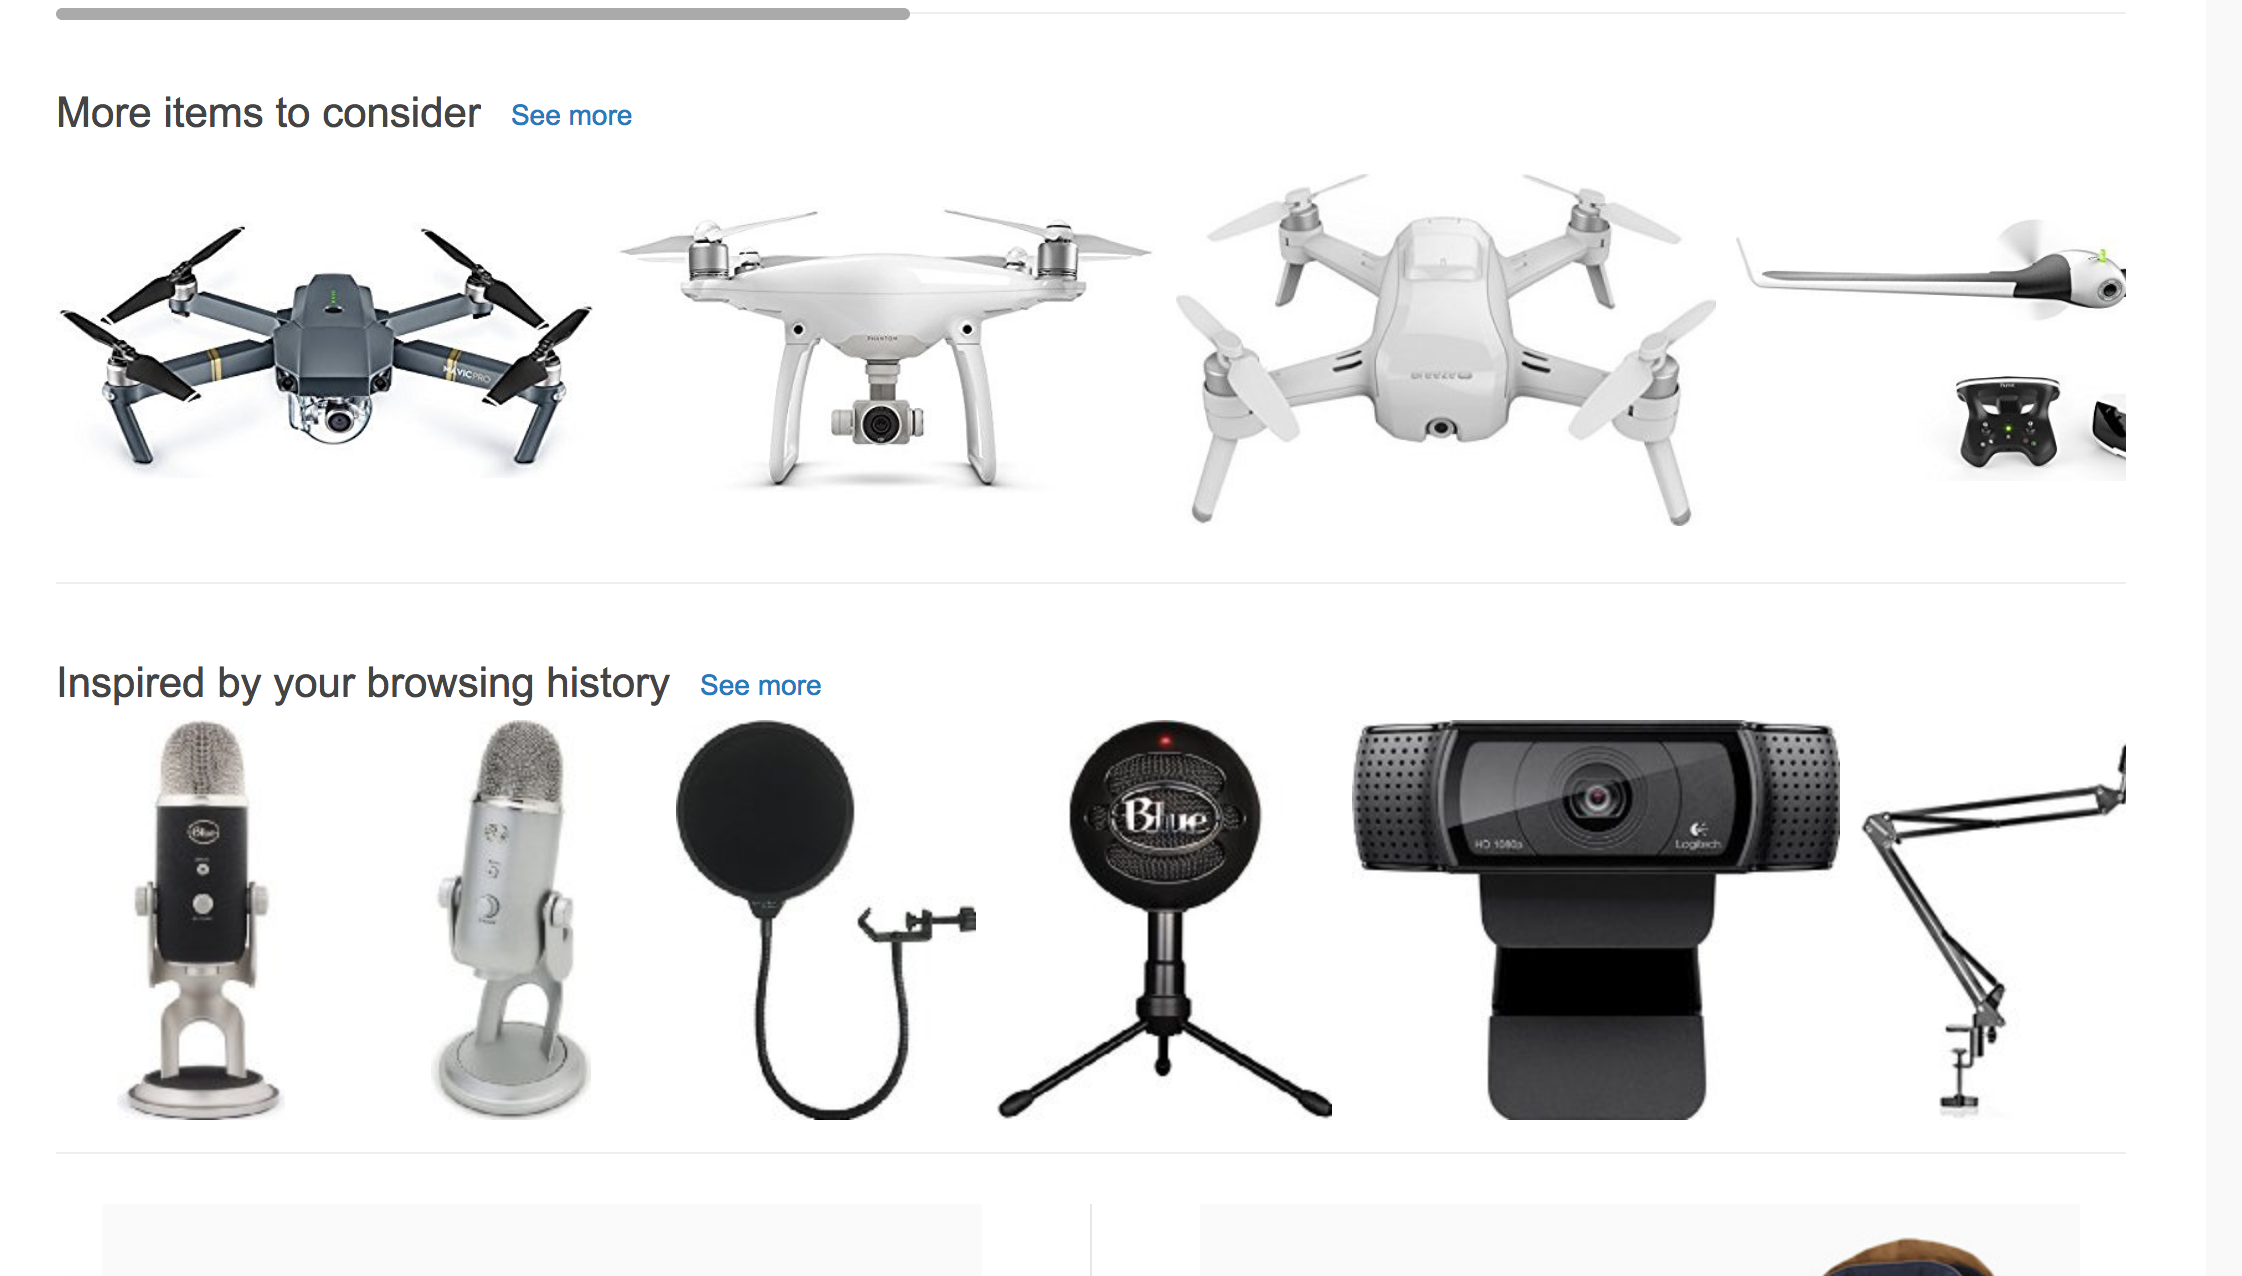
\includegraphics[width=\linewidth]{Images/ml5}
    \end{center}
\end{frame}


\begin{frame}{Motivación}
    \begin{center}
        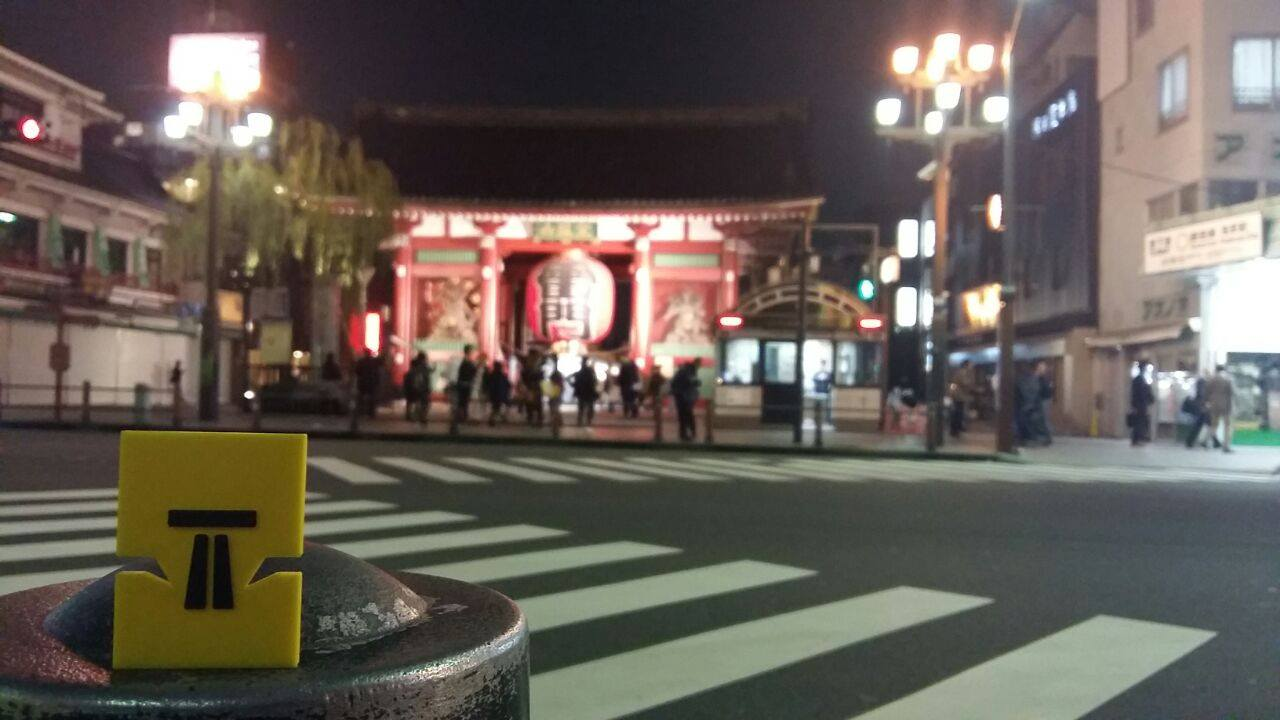
\includegraphics[width=0.9\linewidth]{Images/ml3}
    \end{center}
\end{frame}

\section{Aprendizaje}
\begin{frame}
    \begin{center}
        \large Mejores predicciones
    \end{center}
\end{frame}

\begin{frame}{Inferencia}
    \begin{center}
        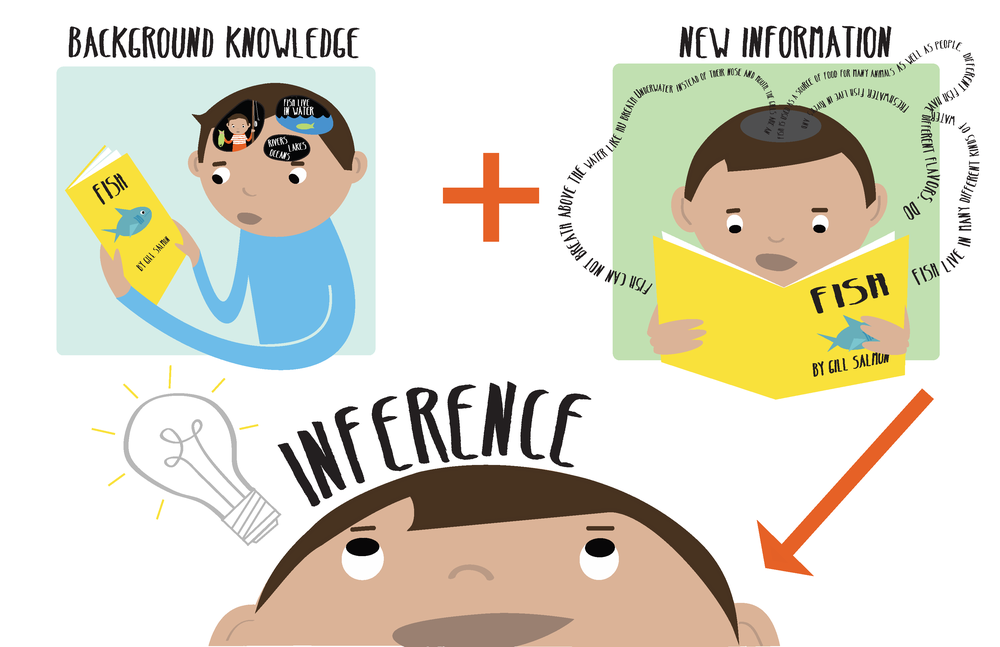
\includegraphics[width=0.9\linewidth]{Images/inferencia}
    \end{center}
\end{frame}

\begin{frame}{Inferencia}
\begin{itemize}
    \item Estadística inferencial (Excel, BI)
    \begin{itemize}
        \item Regresión de datos
        \item Redes bayesianas
    \end{itemize}
    \item \textbf{Aprendizaje de maquina} (Sistemas de recomendación, chatbots)
    \begin{itemize}
        \item Perceptrones
        \item Redes neurales
        \item Clustering
        \item KNN
        \item SNA
    \end{itemize}
\end{itemize}
\end{frame}

\begin{frame}
    \begin{center}
        \large Mejores predicciones
    \end{center}
    \begin{itemize}
        \item Venta (Chatbots, sistemas de recomendación)
        \item Fidelización (Software consciente de contexto, análisis de redes sociales)
        \item Producción (Redes neurales, redes bayesianas)
        \item Análisis (Map-Reduce (aka Big Data))
    \end{itemize}
\end{frame}

\begin{frame}{Netflix}
    \begin{center}
        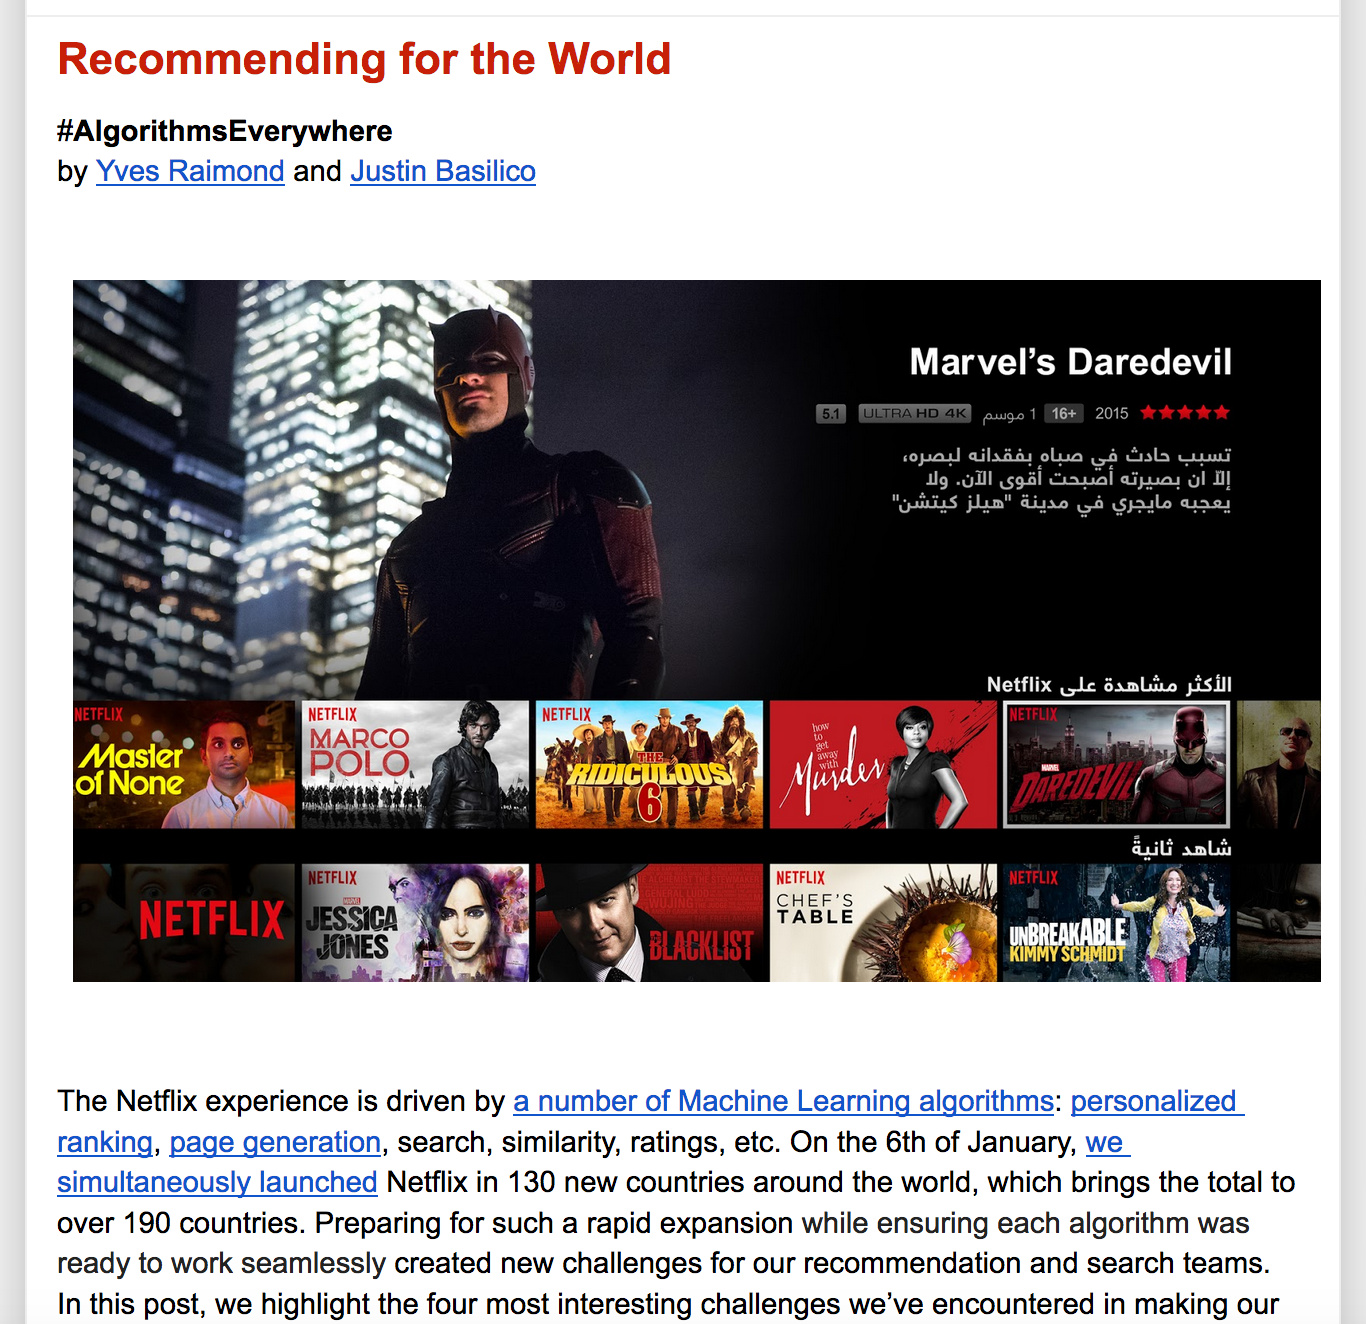
\includegraphics[width=0.9\linewidth]{Images/netflix}
    \end{center}
\end{frame}

\begin{frame}{Inferencia (retos)}
    \begin{itemize}
        \item Problema
        \item Modelo
        \item Implementación
    \end{itemize}
\end{frame}

\subsection{Modelo}
\begin{frame}{1-2-3 Machine Learning}
    \begin{enumerate}
        \item Normalizar los datos
        \item Crear el modelo
        \item Entrenar el modelo
        \item Comprobar su funcionamiento
    \end{enumerate}
\end{frame}

\begin{frame}{Que}
    \begin{itemize}
        \item Probabilidad
        \item Estructura
        \item Conceptos ocultos (Hidden concepts)
    \end{itemize}
\end{frame}

\begin{frame}{Donde}
    \begin{itemize}
        \item Supervised learning (objetivo)
        \item Unsupervised learning (conceptos ocultos)
        \item Reinforcement learning (feedback)
    \end{itemize}
\end{frame}

\begin{frame}{Porque/Para que}
    \begin{itemize}
        \item Predicciones
        \item Diagnostico
        \item Sumarizaciones
    \end{itemize}
\end{frame}

\begin{frame}{Como}
    \begin{itemize}
        \item Pasivo (Observador)
        \item Activo
        \item Offline
        \item Online
    \end{itemize}
\end{frame}

\begin{frame}{Salida}
    \begin{itemize}
        \item Clasificación (Binario)
        \item Regresión (Continuo)
    \end{itemize}
\end{frame}

\begin{frame}{Detalles}
    \begin{itemize}
        \item Generativo (Generalizaciones)
        \item Discriminativo (Distinguir)
    \end{itemize}
\end{frame}

\begin{frame}{Navaja de Occam}
    \begin{center}
        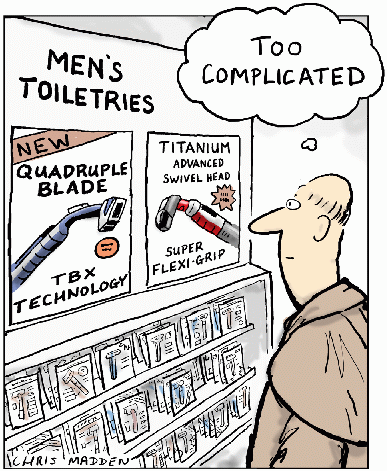
\includegraphics[width=0.7\linewidth]{Images/occam}
    \end{center}
\end{frame}

\begin{frame}{Navaja de Occam}
    "Pluralitas non est ponenda sine necessitate"
    
    "Plurality is not to be posited without necessity"
\end{frame}

\begin{frame}{Navaja de Occam (Español)}
    Cuando se tienen dos teorias que obtenen las mismas predicciones, generalmente la más simple es la mejor
\end{frame}



\subsection{Implementación}
\begin{frame}{Bibliotecas}
    Principales
    \begin{itemize}
        \item DeepLearning4J \url{https://deeplearning4j.org/}
        \item BID Data Project \url{http://bid2.berkeley.edu/bid-data-project/}
        \item Neuroph \url{http://neuroph.sourceforge.net/index.html}
                \item Smile \url{http://haifengl.github.io/smile/}
    \end{itemize}

    Complementarias
    \begin{itemize}
        \item Commons Math \url{http://commons.apache.org/proper/commons-math/}
        \item Eclipse Collections \url{https://www.eclipse.org/collections/}
    \end{itemize}
\end{frame}

\begin{frame}{Paas}
    \begin{itemize}
        \item AmazonML \url{https://aws.amazon.com/machine-learning/}
        \item Bluemix - Watson \url{https://www.ibm.com/cloud-computing/bluemix/watson}
        \item Oracle Advanced Analytics \url{https://www.oracle.com/database/advanced-analytics/index.html}
    \end{itemize}
\end{frame}


\section{Demo}
\begin{frame}{Demo}
    \begin{enumerate}
        \item Mamiferos
        \item Aves
        \item Sangre fria
        \item Pez
        \item Anfibios
        \item Insectos
        \item Maritimo
    \end{enumerate}
\end{frame}

\begin{frame}{Demo}
    \begin{enumerate}
        \item Cabello
        \item Plumas
        \item Huevos
        \item Leche
        \item Volador
        \item Acuatico
        \item Depredador
        \item Dientes
        \item Columna vertebral
        \item Respira
        \item Venenoso
        \item Aletas
        \item Cantidad piernas
        \item Cola
        \item Domestico
        \item "Tamaño gato"
   \end{enumerate}
\end{frame}

\begin{frame}{Demo}
    \begin{enumerate}
        \item Learning rate: Velocidad de aprendizaje
        \item Momentum: Controla convergencia hacia minimos
        \item Error: Mientras menor sea el error, mayor la aproximación*
    \end{enumerate}
\end{frame}

\section{Experiencias previas}

\begin{frame}{JRiskSimulator}
    \begin{itemize}
        \item \textbf{Problema:} Mejorar las recomendaciones en ISO 27001
        \item \textbf{Modelo: } Clasificación inmediata mediante análisis de redes sociales
        \item \textbf{Implementación: }  JGraph + JUNG + Commons Math + Java FX
    \end{itemize}
\end{frame}

\begin{frame}{JRiskSimulator}
    \begin{center}
        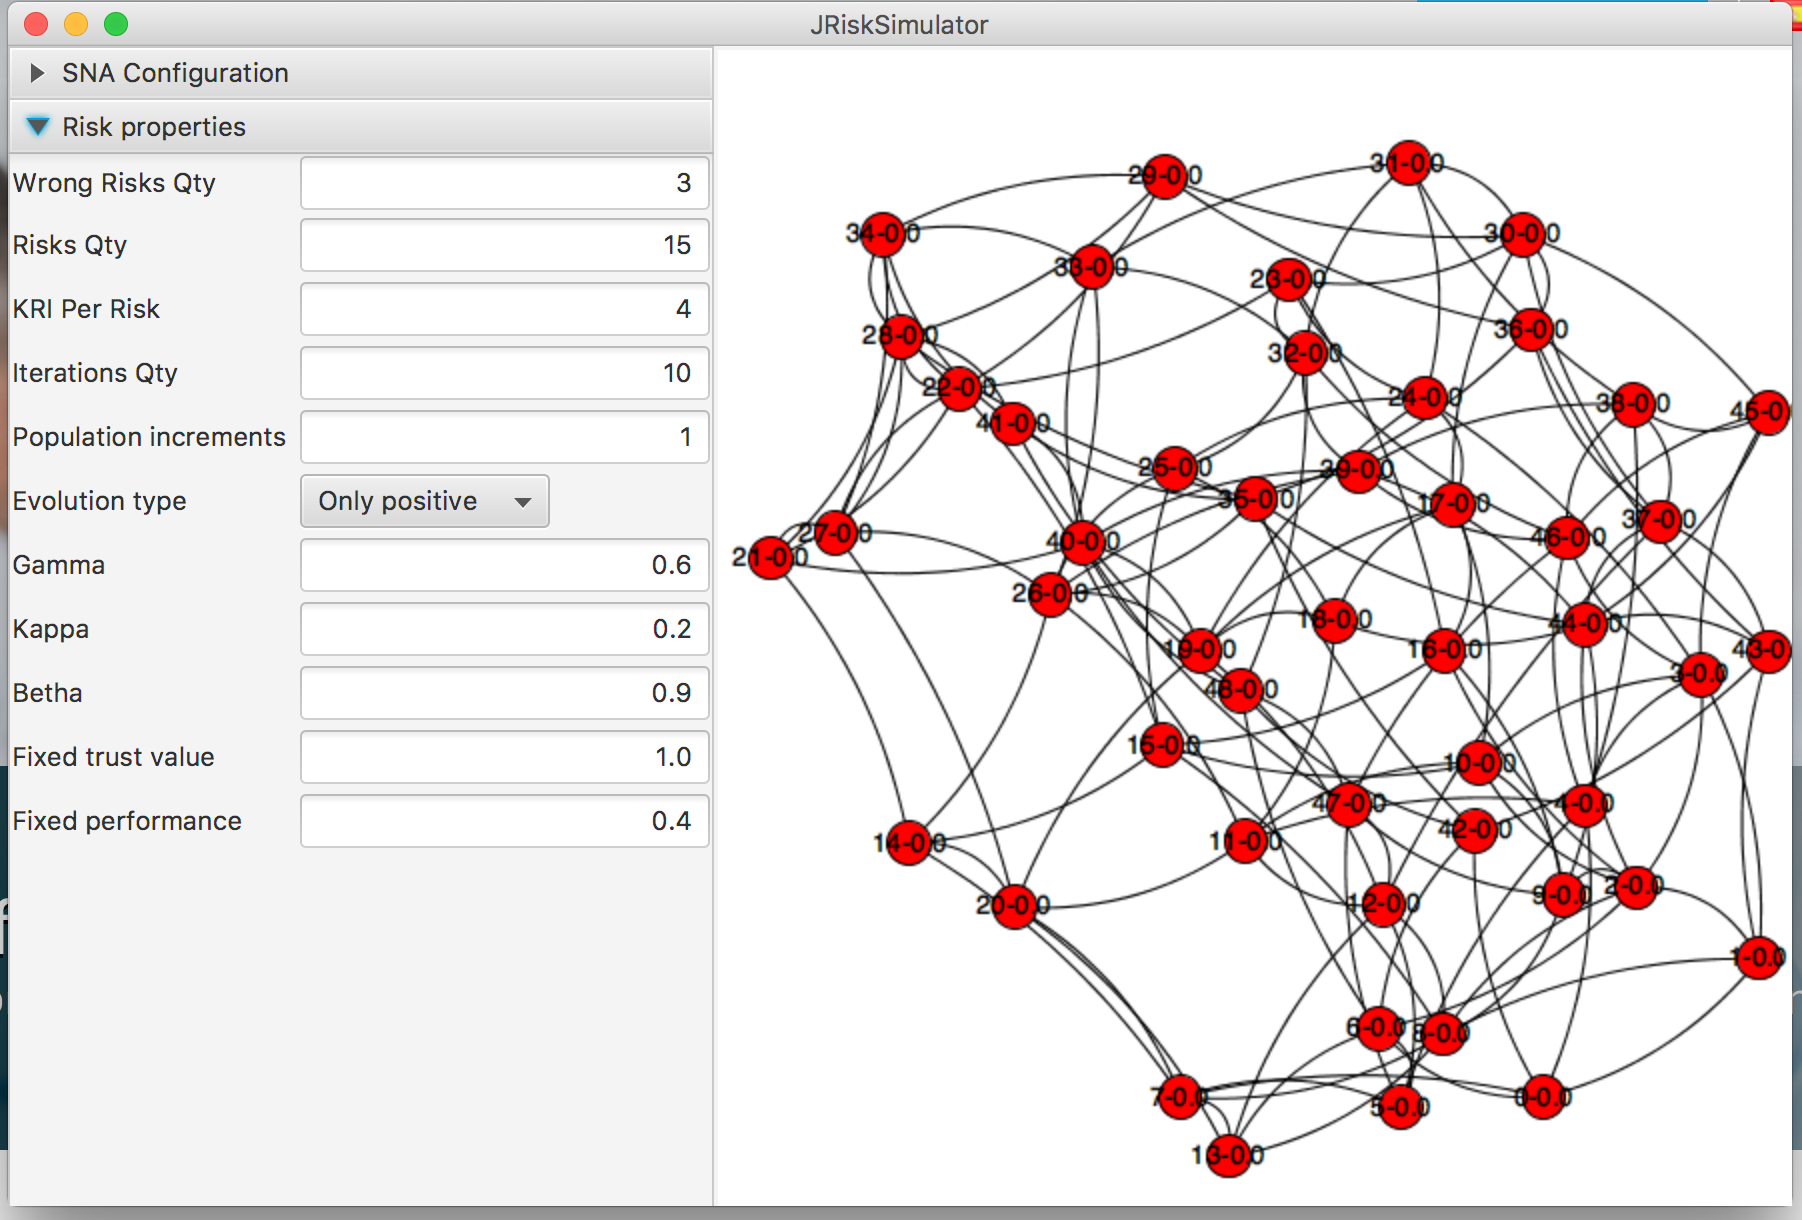
\includegraphics[width=0.9\linewidth]{Images/jrisk}
    \end{center}
\end{frame}

\begin{frame}{Medmigo}
    \begin{itemize}
        \item \textbf{Problema:} Adaptar la recomendación de un profesional de acuerdo a las recomendaciones de mis amigos
        \item \textbf{Modelo: } Clasificación inmediata mediante perceptrones + Análisis de redes sociales
        \item \textbf{Implementación: } Neuroph + Commons Math + Lucene Search + Java EE 
    \end{itemize}
\end{frame}

\begin{frame}{Medmigo}
    \begin{center}
        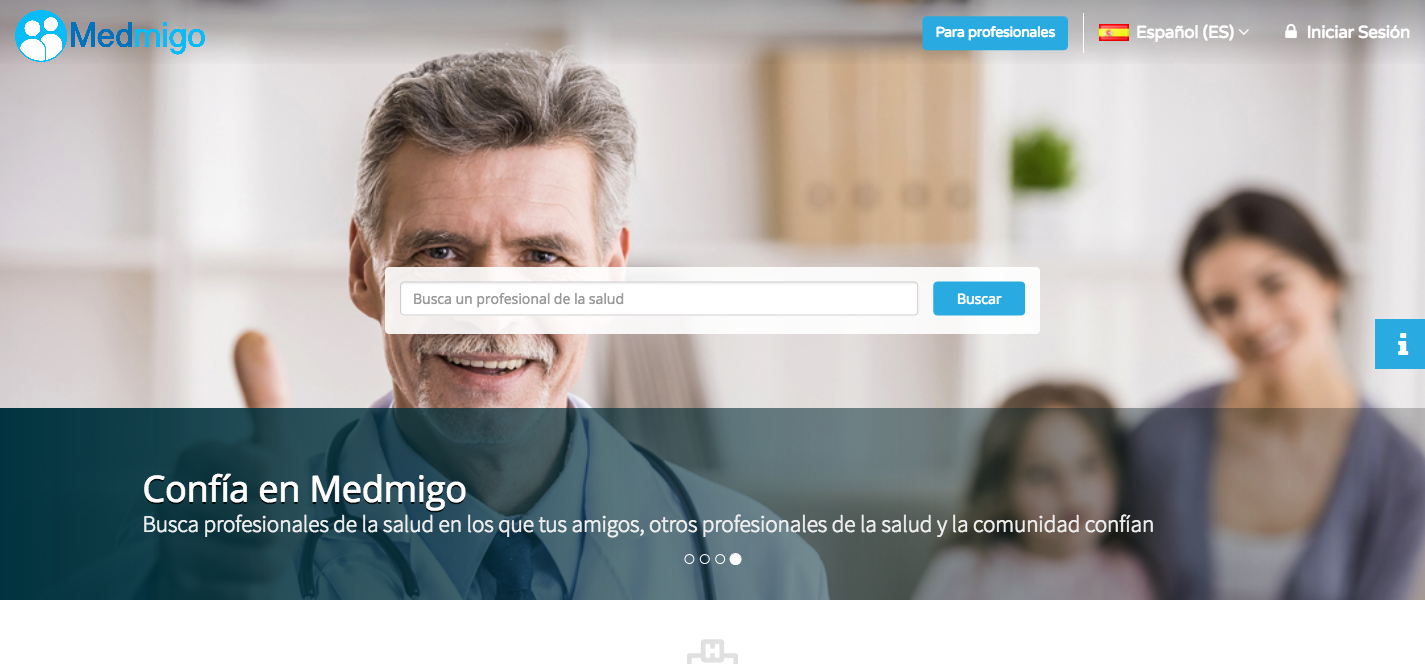
\includegraphics[width=0.9\linewidth]{Images/Medmigo}
    \end{center}
\end{frame}

\begin{frame}{SGB - Bible Generation}
    \begin{itemize}
        \item \textbf{Problema:} Indexar n cantidad de biblias en un metabuscador que soporte "palabras parecidas"
        \item \textbf{Modelo: } Binary tree + Tokenization + Levenshtein distance + Lazy data fetch
         \item \textbf{Implementación: } Lucene Search + Java EE 
    \end{itemize}
\end{frame}

\begin{frame}{SGB - Bible Generation}
    \begin{center}
        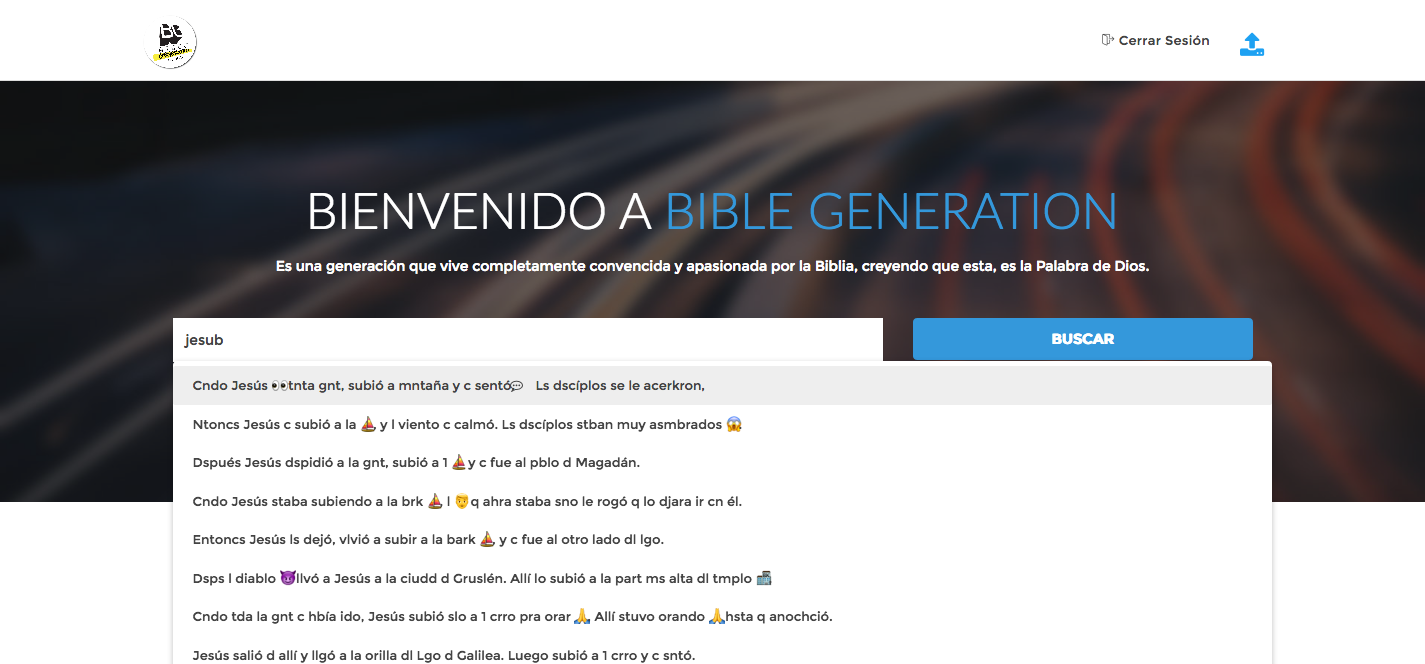
\includegraphics[width=0.9\linewidth]{Images/bible}
    \end{center}
\end{frame}


\section{Fin}

\begin{frame}{Gracias}
\begin{itemize}
\item me@vorozco.com
\item http://vorozco.com
\item http://github.com/tuxtor/slides
\end{itemize}
\begin{center}

\includegraphics[width=0.1\linewidth]{Images/cclogo}
\\
This work is licensed under a Creative Commons Attribution-ShareAlike 3.0 Guatemala License.
\end{center}
\end{frame}
\end{document}

